%Un exercice avec son corrigé à inclure dans un fichier principal.

\exo{Étude de fonction}

Soit $f$ la fonction définie sur $[6; 30]$ par $f(x) = \dfrac{1}{2}x^2 - 36 \ln x + 150$.

On note $\mathcal{C}$ la courbe représentative de $f$ dans un repère orthogonal $\left(O ; \overrightarrow{i} ; \overrightarrow{j} \right)$. On prendra comme unités graphiques : 1 cm pour 5 sur l'axe des abscisses et un centimètre pour 100 sur l'axe des ordonnées.

 \question{Dérivée}

 \subquestion{}
 Montrer que, pour tout nombre réel $x$ de $[6;30]$,

\begin{equation*}
f'(x) = \dfrac{(x+6)(x-6)}{x}
\end{equation*}

\correction{
\begin{equation*}
f'(x) = x - \dfrac{36}{x} = \dfrac{x^2 - 36}{x} = \dfrac{(x+6)(x-6)}{x}
\end{equation*}
}

 \subquestion{}
 Étudier le signe de $f'(x)$ lorsque $x$ varie dans $[6;30]$.

\correction{
Sur $[6;30]$, $x>0$, $x+6>0$ et $x-6 \geqslant 0$, donc $f'(x) \geqslant 0$ sur $[6;30]$.
}

 \subquestion{}
 En déduire la tableau de variation de $f$ sur $[6;30]$.

\correction{
\begin{center}
\begin{tikzpicture}
   \tkzTabInit{$x$ / 1 , $f(x)$ / 2}{$6$, $30$}
   \tkzTabVar{-/ $103$, +/ $478$}
\end{tikzpicture}
\end{center}
}

 \question{Tracé de la courbe}

 \subquestion{}
Compléter, après l'avoir reproduit sur la copie, le tableau de valeurs suivant dans lequel les valeurs approchées sont à arrondir à l'unité.

\begin{center}
\begin{tabular}{|c|c|c|c|c|c|c|}
\hline
$x$    & 6 & 10 & 15 & 20 & 25 & 30 \\ \hline
$f(x)$ & \hspace{15mm}  &  \hspace{15mm}  &  \hspace{15mm}  &  \hspace{15mm}  &  \hspace{15mm}  &  \hspace{15mm}  \\ \hline
\end{tabular}
\end{center}

\correction{
\begin{center}
\begin{tabular}{|c|c|c|c|c|c|c|}
\hline
$x$    & 6    & 10    & 15   & 20  & 25  & 30 \\ \hline
$f(x)$ & 103  &  117  & 165  & 242 & 347 & 478 \\ \hline
\end{tabular}
\end{center}
}


 \subquestion{}
 Tracer la courbe $\mathcal{C}$ dans un repère sur la copie.

\correction{
\begin{center}
\simpleplot{6}{30}{\x}{0.5*(\x)^2 - 36*ln(\x) + 150}{$\mathcal{C}_f$}{1}
\end{center}
}

